\documentclass{article}
\usepackage[utf8]{inputenc}
\usepackage{array}
\usepackage{amsmath,amssymb}
\usepackage{booktabs}
\usepackage{caption}
\usepackage[nodayofweek]{datetime}
\usepackage{environ}
\usepackage{float}
\usepackage{enumitem}
\usepackage{fancyhdr}
\usepackage[margin=25mm,footskip=20pt,includefoot]{geometry}
\usepackage{graphicx}
\usepackage{hyperref}
\usepackage{multicol}
\usepackage{rotating}
\usepackage{tikz}
\usepackage{threeparttable}
\usepackage{url}
\usepackage{xspace}
\usepackage{bm}
\usepackage{lipsum}


\hypersetup{
    colorlinks=true,
    urlcolor=blue}

\begin{document}
\noindent
\textbf{ES280 Problem Set 2} \\
\textbf{Nick Normandin} \\
\section*{Classmates consulted}
I consulted Kaelyn, Sophie, and Daniel on this problem set.

\section{Uniform colors}%
\label{sec:Uniform colors}

\subsection{One-sided vs. two-sided tests}%
The researchers would likely use a two-sided test in this case because they do not appear to have a prior belief about one color having a higher probability of winning than the other. They state that the problem is to determine whether "one of the colors will win a majority of the time", which indicates that they are looking for any deviation from the expected probability of $0.5$. One implication of using a two-sided test is that it will increase the p-value.
\label{sub:One-sided vs. two-sided tests}
\begin{enumerate}[label=\alph*.]
    \item The null hypothesis $H_0$ is that the probability of a competitor wearing red winning is equal to $0.5$. The alternative hypothesis $H_a$ is that the probability of the competitor wearing red winning is greater than $0.5$.
    \item $H_0: p = 0.5, \quad H_a: p > 0.5$
    \item Since the number of samples is large ($n>>40$) we will use the Z statistic. 
        $$Z = \frac{\hat{P} - p - \Delta_\mu}{\sqrt{p(1-p)/n}}=\frac{0.543 - 0.5 - 0}{\sqrt{0.5(1-0.5)/457}}=1.82$$
    \item We could use a binomial distribution (a series of coin flips) to simulate this same experiment. We could flip a fair coin ($p(heads)=0.5$) 457 times and count the number of heads (successes). We could run this simulation thousands of times, creating an empirical PMF out of the proportion of successes observed. We could then sum the portion of the PMF that is as or more extreme than a success rate (rate of seeing heads) $54.3\%$ of the time. Since the number of heads out of 457
        flips is countably finite, we could use a discrete distribution.
    \item Entering \texttt{1-normcdf(1.82)} into Matlab yields a p-value of 0.0341. My conclusion is that we can reject the null hypothesis with fairly good certainty. Within the context of our experiment, we would reject the null hypothesis that the likelihood of a competitor wearing red will win $50\%$ of matches.
        $$ N \sim(0.5, 0.0234)$$
    \item See Figure 1.
\begin{figure}[ht]
\begin{center}
    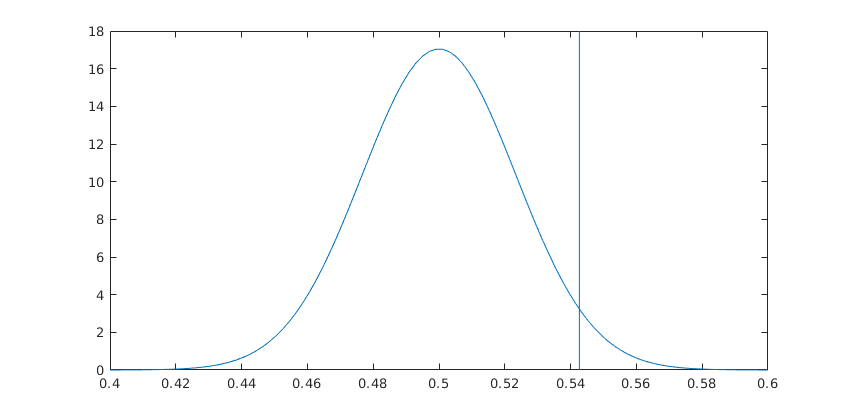
\includegraphics[scale=0.2]{fig1}
    \caption{Plot of null distribution}
\end{center}
\end{figure}
    \item The null hypothesis $H_0$ is that the probability of a competitor wearing red winning is equal to $0.5$. The alternative hypothesis $H_a$ is that the probability of the competitor wearing red winning is not equal to $0.5$.
        $$H_0: p = 0.5, \quad H_a: p \neq 0.5$$
    \item From \texttt{2*(1-normcdf(Z))} in Matlab, we get a p-value of $0.0681$ which is double the one-sided p-value.
    \item See Figure 2.

\begin{figure}[ht]
\begin{center}
    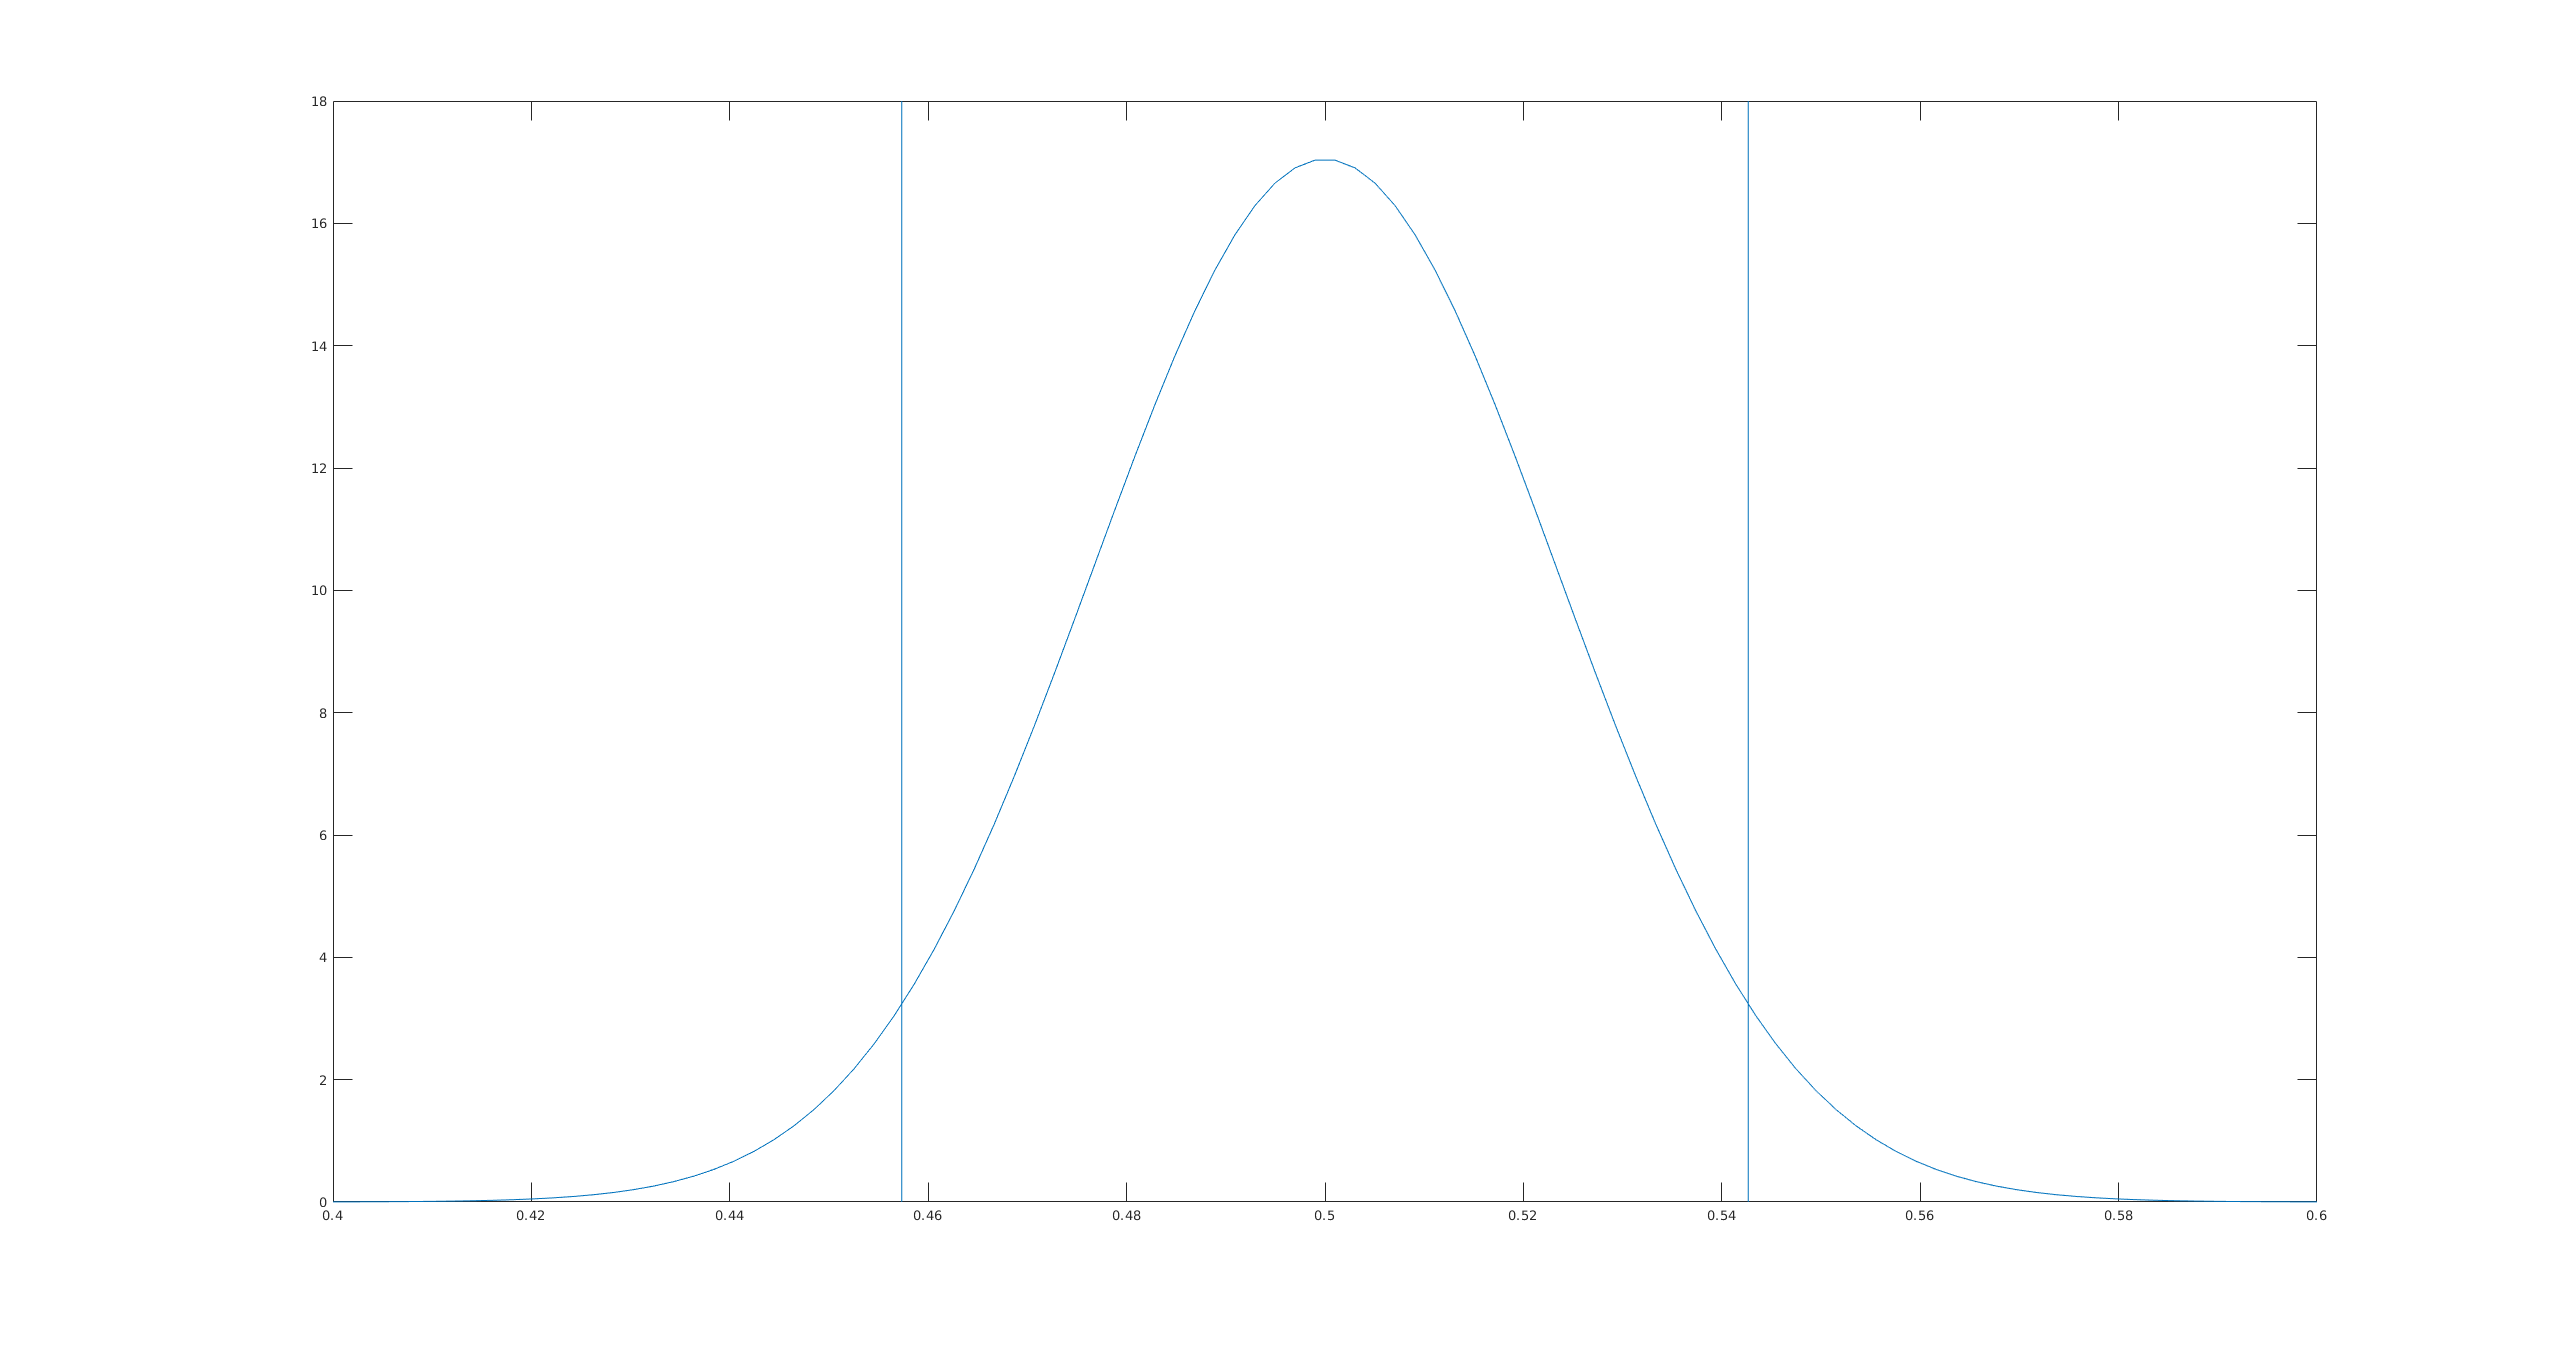
\includegraphics[scale=0.2]{fig1b}
    \caption{Plot of null distribution}
\end{center}
\end{figure}
    \item Moving from a one-sided to a two-sided test increases the difficulty of rejecting the null hypothesis. This is because your p-value is doubled in a two-sided test. 

\end{enumerate}

\subsection{Effect size}%
\label{sub:Effect size}
\begin{enumerate}[label=\alph*.]
    \item  In this case, the test statistic is:
        $$Z = \frac{\hat{P} - p - \Delta_\mu}{\sqrt{p(1-p)/n}}=\frac{0.57 - 0.5 - 0}{\sqrt{0.5(1-0.5)/457}}=2.99$$
        The new one-sided p-value is 0.0014 and the two-sided p-value is 0.0028.
    \item They are smaller. The difference between the ratio $\hat{P}$ and the value of $p$ under our null hypothesis has grown, so we should have more confidence in rejecting $H_0$.

    \item The distance between the observed paramter $\hat{P}$ and the value specified under the null hypothesis, $p$, is in the numerator of the function which calculates our Z-score. This means that a larger value of $\hat{P}-p$ (assuming $\Delta_0$ does not change) will result in a larger Z score, and a smaller p-value.

\end{enumerate}

\subsection{Sample size}%
\label{sub:Sample size}
\begin{enumerate}[label=\alph*.]
    \item The mean is still 0.5 but the standard deviation has increased by nearly 50\% to 0.0303.
    \item  In this case, the test statistic is:
        $$Z = \frac{\hat{P} - p - \Delta_\mu}{\sqrt{p(1-p)/n}}=\frac{0.551 - 0.5 - 0}{\sqrt{0.5(1-0.5)/272}}=1.6977$$
        The new one-sided p-value is 0.0448 and the two-sided p-value is 0.0896. These p-values are larger than the original case, which makes sense given the decrease in sample size.
    \item Even though the effect size has actually increased, the decrease in the number of samples taken makes it more difficult for us to reject $H_0$.
\end{enumerate}

\section{Sampling distribution}%
\label{sec:Sampling distribution}
\begin{enumerate}[label=\alph*.]
    \item We can calculate a Z-statistic using the standard error, which is $1.0/\sqrt{25} = 0.2$.
        $$ Z = \frac{x - \mu}{\sigma} = \frac{3.25 - 3.5}{0.2}=-1.25$$
    From Matlab, \texttt{1- tcdf(-1.25, 24) = 0.8944}.
    \item We can calculate a Z-statistic using the standard error, which is $1.0/\sqrt{25} = 0.2$.
        $$ Z = \frac{x - \mu}{\sigma} = \frac{3.25 - 3.5}{0.1}= -2.5$$
    From Matlab, \texttt{1- tcdf(-1.25, 24) = 0.9938}.
    \item The last two probabilities differ because increasing our sample size decreases our standard error.
\end{enumerate}


\section{Executive}%
\label{sec:Executive}
\begin{enumerate}[label=\alph*.]
    \item Where $x$ is defined as length of employment in years, $H_0: x \geq 6, \quad H_a: x < 6$.  
        $$ T = \frac{\bar{x} - \mu}{s/\sqrt{n}} = \frac{5.25-6}{1.5/\sqrt{6}}=-1.4697$$
    We should fail to reject the null hypothesis because the $T_{reject}$ value is -2.015.
\item The p-value from Matlab is \texttt{tcdf(-1.4697, 6-1) = 0.1008}. 
\end{enumerate}

\section{Lottery}%
\label{sec:Lottery}
\begin{enumerate}[label=\alph*.]
    \item With $x_1$ as the array of states with `For Education' and $x_2$ as the array of states with `General Use', we can use Matlab to determine that we fail to reject the null hypothesis.\\ \\ 
        In Matlab, \texttt{ttest2(x1, x2, `vartype', `equal', `Tail', `right')} yields $p=0.0481$.
\end{enumerate}

\section{Stomach flu}%
\label{sec:Stomach flu}
\begin{enumerate}[label=\alph*.]
    \item We can calculate the test statistic using:

        $$Z = \frac{\hat{p}_1 - \hat{p}_2}{\sqrt{\hat{p}(1-\hat{p})(\frac{1}{n_1}+\frac{1}{n_2})}} = \frac{0.43 - 0.36}{\sqrt{0.38(1-0.38)(\frac{1}{55}+\frac{1}{149})}}= 0.9645$$

        The critical Z-value is 1.65. We therefore fail to reject the null hypothesis.
    \item Matlab yields a p-value of \texttt{1-normcdf(0.9645)}= 0.1674.
\end{enumerate}

\section{Matlab problem}%
\label{sec:Matlab problem}
\begin{enumerate}[label=\alph*.]
    \item See Figure 3.
\begin{figure}[ht]
\begin{center}
    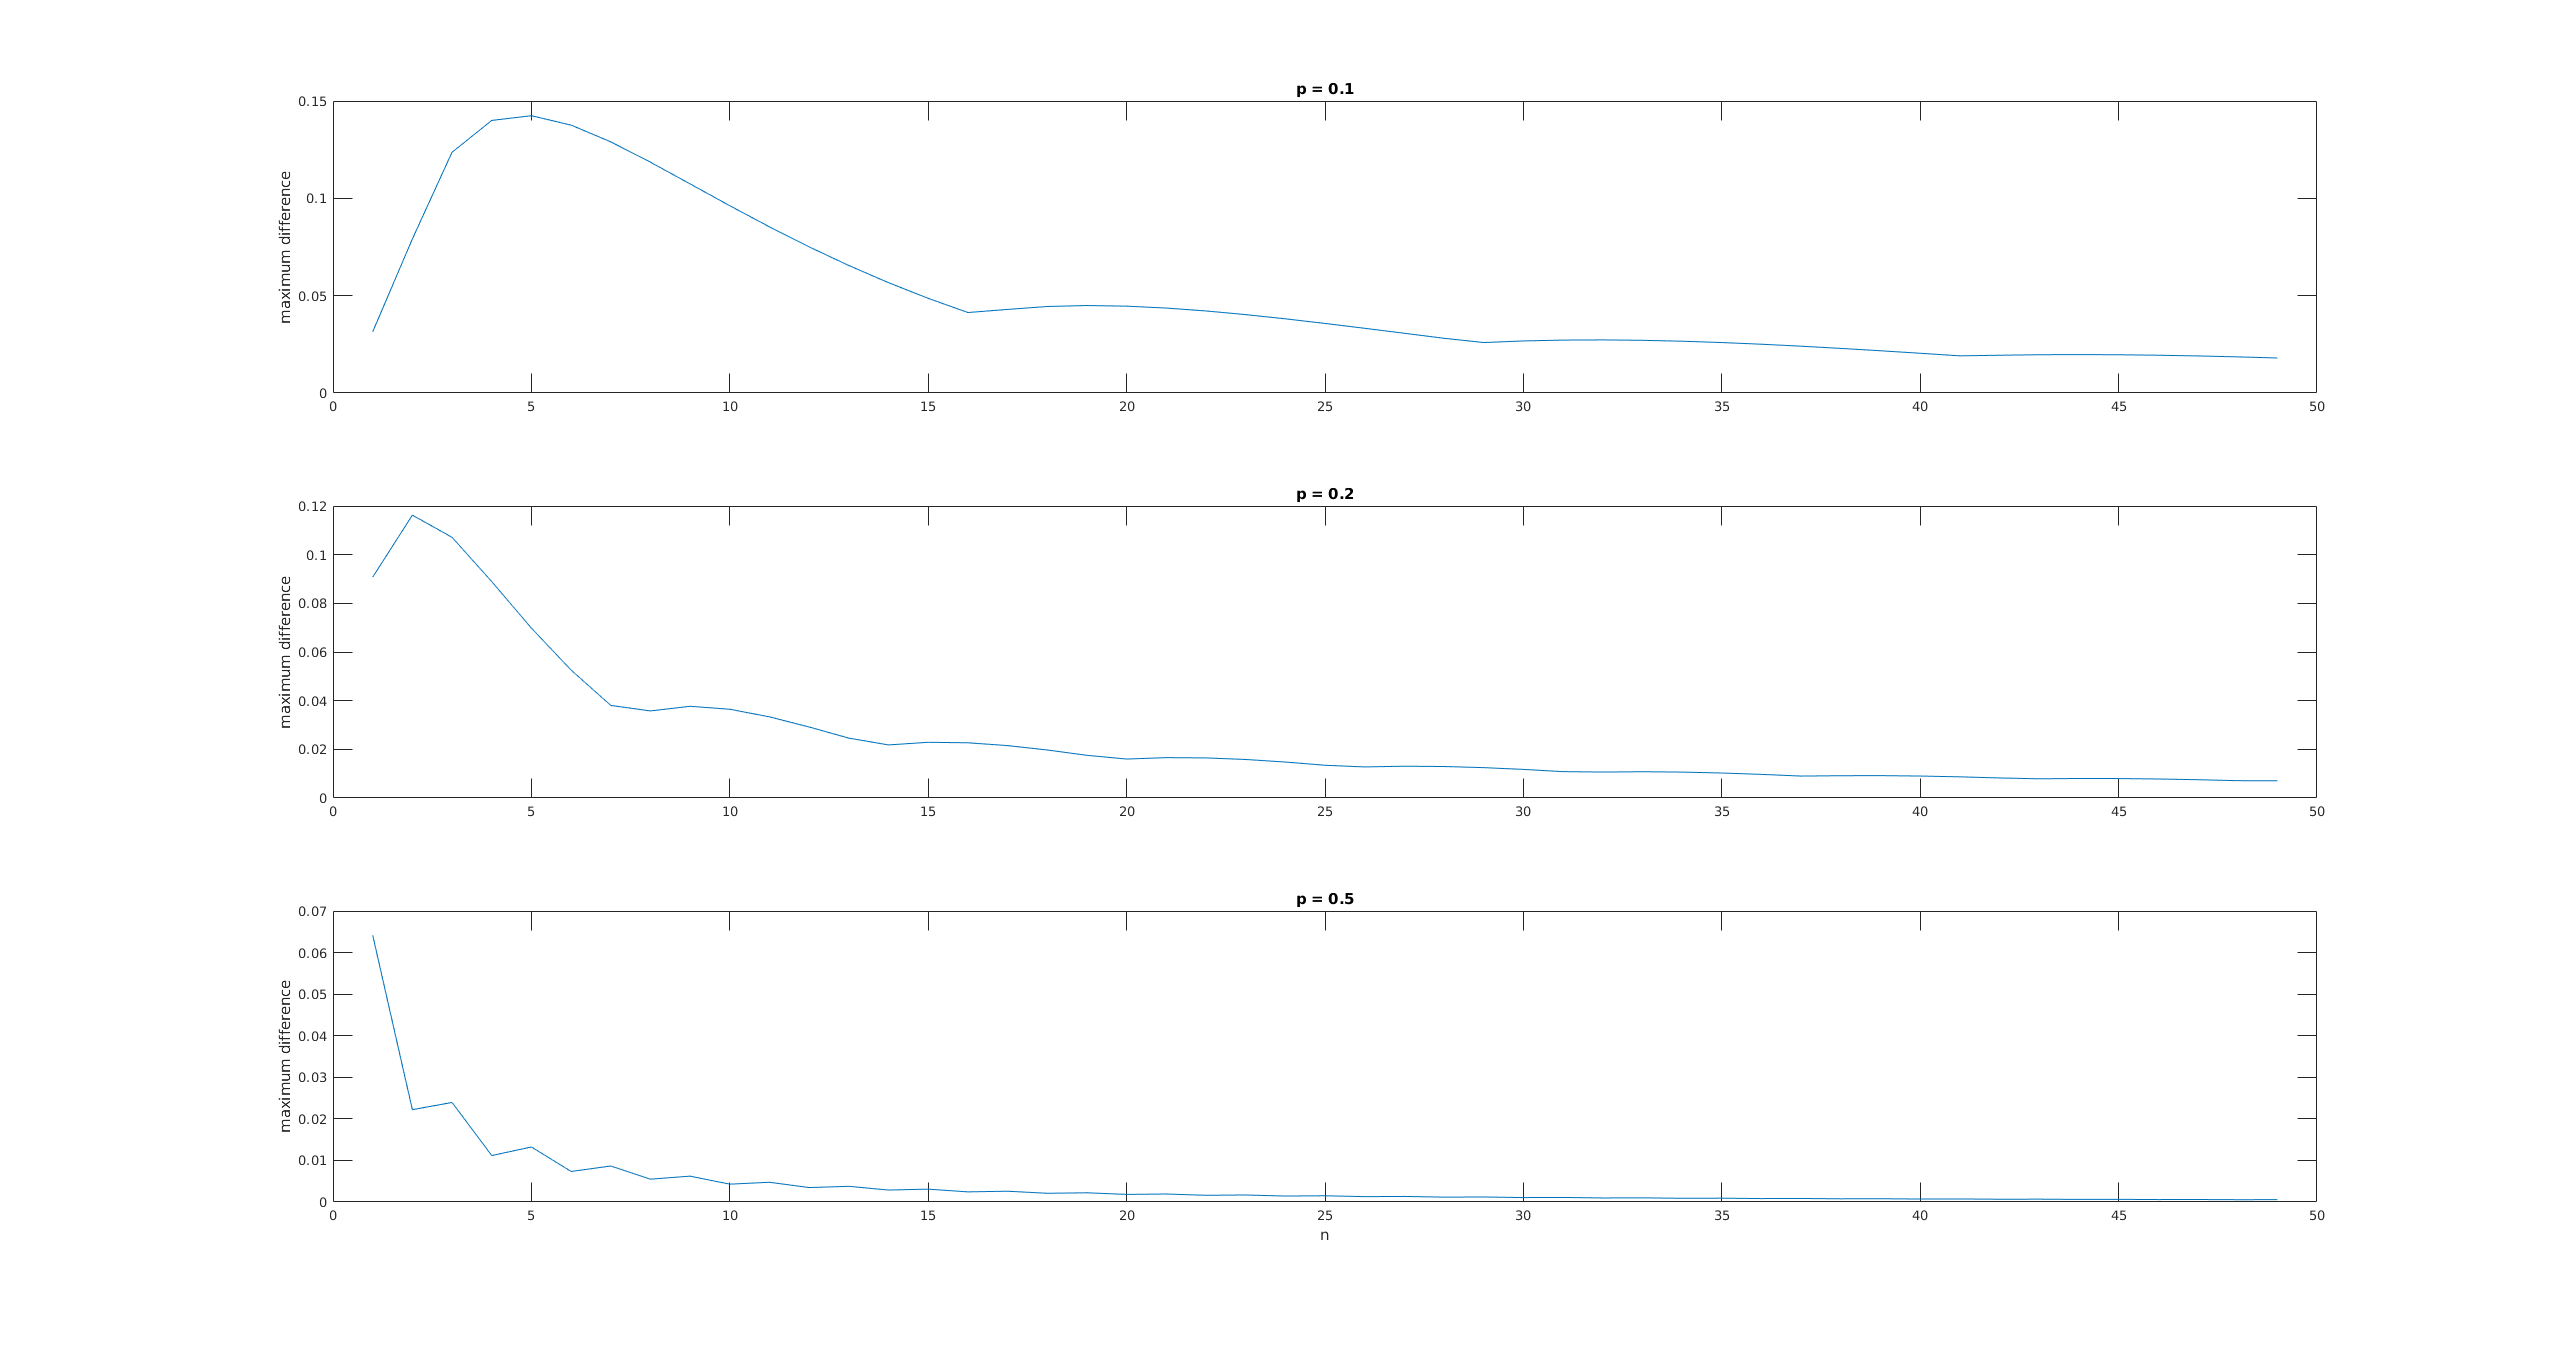
\includegraphics[scale=0.29]{fig2}
    \caption{Plot of binomial and normal max differences}

\end{center}
The maximum value when both $np>5$ and $n(1-p)>5$ .
\end{figure}
\end{enumerate}


% \begin{figure}
% \begin{center}
%     \includegraphics[scale=0.28]{ps1_hist}
% \end{center}
% \end{figure}


\end{document}
